\documentclass{article}
\usepackage{graphicx}
% \usepackage[%
% 	colorlinks=true
% 	pdfborder={0,0,0}
% 	linkcolor=blue
% ]{hyperref}
\graphicspath{{images/}}
\title{D and D Finder Architecture}
\author{Sean Calkins \\ Linh \\ Ryeland Ellison}
\date{Spring 2024}
\begin{document}
	\begin{figure}
		\centering
		
\includegraphics[width=0.85\textwidth]{dd_dragon.png}
	\end{figure}

\maketitle
\newpage
%///////////////////////////////////////////////////////////////////////////////////////////////////
	\section{Introduction}
	This document describes the architecture of the D and D finders application. As a brief 
	overview, the application is used by prospective Dungeons and Dragons players who do not
	have a D and D group. This app allows them to connect with other D and D players to form
	a group.
	The purpose of this document is to give developers in the future documentation to follow if they
	are to pursue further development of this project. The document will mainly be broken into the 
	3 main layers mobile application development: The data layer, the application layer, and the logic
	layer. The logic layer will not have it's own section because it is the glue that holds together 
	the data and application layer, so it will be mentioned during discussion of the other layers. 

	\newpage

	\section{Data Layer}
	This type of application requires an advanced back end to store massive amounts of relational
	data, however we took a different approach. Instead of connecting the back end to a database,
	we stored all the data in a single JSON object that can be pushed pulled from a remote 
	location. There are benefits and draw backs to this approach. One of the benefits is
	the simplicity of implementation. Instead of creating an entire backend relational database,
	which could take a long time to implement, the simple JSON object is quick and easy. Another 
	benefit is the speed of retrieving data in the JSON structure. JSON files in Javascript are 
	hashmaps, so accessing values from the map based on a key is quick and easy. 
	There are several drawbacks however, such as having to fetch all the data anytime there is a fetch.
	This scales poorly for having a lot of users. 

	% Change Figure 1 to be a link if you are feeling spicy
	Figure 1 shows the interaction between the remote, the application, and the backend. 
	The remote speaks to the backend via the javascript fetch function. This is an asynchronous
	function that can perform POST and GET requests to a remote server. This requesting of data via
	fetch is handled with a javascript component in the application. 
	Due to the backend having to fetch the data asynchronously, the application must communicate with
	backend asynchronously. React Native handles this situation very well. At first it seems silly
	because React Native doesn't have support for initialization of asynchrounous data in components, 
	however this was intentionally. To properly use an asynchronous component, the developer is envouraged
	to always have a default case for when we are waiting for the data asynchronously. For example, if
	we make a request to get the JSON from the server to display the current user, then while we wait 
	for the data, we can display a default Jane Doe user. After we get the data, we can update the Jane 
	Doe to dispaly the requested user. This will keep the app responsive for the user, and typically
	the response happens fast enough that the user never sees the Jane Doe profile in the first place. 



	\begin{figure}[b]
		\centering
		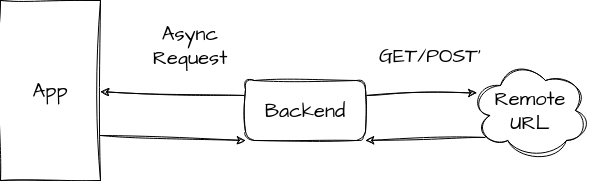
\includegraphics[width=1\textwidth]{remote.png}
		\caption{This figure shows the interaction between the remote, the application and the
		backend.}
	\end{figure}

	\newpage


	\section{JSON Data Storage}
	In the previous section, we learned that the data structure for our architecture was a singular
	JSON object. This JSON structure is organized as an array of character profiles. Each character
	profile has many attributes that describe them, including but not limited to their character
	name, class, age, and race. The JSON also contains meta data, such as which characters that a 
	specific character has liked or disliked in the past and the characters status.

	The code snipped below is an example of what one of the character JSON object looks like.
	There are a couple things to note. The first thing is the password. Currently the password is 
	stored in plain text, however a future release of this application should include hashing the
	password before storing it in the JSON. The next time the user logs in, we simply hash their guess
	and compare the hashes. If they match hashed that means that they are the same unhashed. 
	Many fields were taken out in this specific example for simplicity.

	\begin{verbatim}
  {
    id: 1,
    email: "l@gmail.com",
    password: "123456",
    firstname: "Leane",
    charactername: "Leanne Stormcloak",
    characterClass: "paladin",
    characterLevel: "20",
    campaign: "Elf home",
bio: "upstanding paladin who fights for the little guy. I love to swing my big ass sword around ",
    otheruser: [],
    like: [2, 5],
    dislike: [],
    match: [2],
  }
	\end{verbatim}

	\newpage
	\section{Application Layer}
	This layer of the architecture diagram describes the application layer of the App. This layer
	includes architecture of the components that make up the interface and logic of the application as a
	whole. 

	The figure below describes the interaction between the main applicaiton layer components. The application 
	is defined by an initial App.js, which is broken into several smaller components. These are the main
	components and interfaces of the application. Each of these components further breaks down into smaller
	components, however we will not go into that level of detail for the sake of simplicity within this
	document. 

	The main App component breaks into 2 pieces: the Login and Navbar components. If the logic layer
	of the application detects that the user isn't logged in, then the Login component will be ran and
	displayed. If the user is logged in, then the NavBar component takes effect. 

	The NavBar component is responsible for housing the 3 main components of the application: the Home
	component, the Chat component, and the Profile component. Each of these components represents a
	major interface of the application. The Home component is where users will spend the majority of 
	their time, scrolling through other D and D users. When the user scrolls through other character
	profiles, the backend will fetch the required data and update if there have been changes. The Chat
	component is where users will chat with other users. This component is the most difficult for the
	backend, as is it updated more frequently then the other components. The final major component is
	the Profile. This is where the user can update their D and D character, which will then be saved 
	to the remote. 

	\begin{figure}[b]
		\centering
		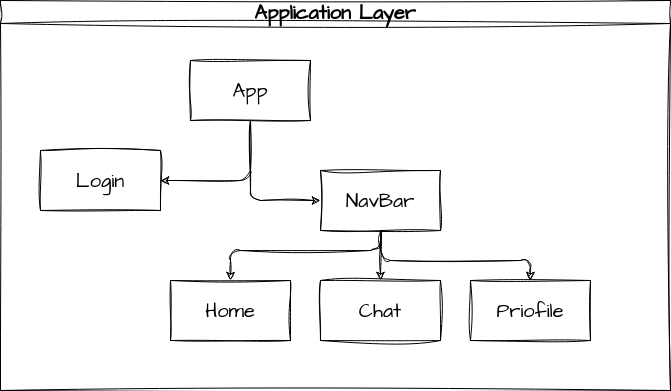
\includegraphics[width=0.6\textwidth]{app-layer.png}
		\caption{This figure shows the interaction between the main application layer components.}
	\end{figure}

%///////////////////////////////////////////////////////////////////////////////////////////////////
\end{document}
